\documentclass[../thesis-main.tex]{subfiles}

\begin{document}

\chapter{Isch\ae{}mic Variation}
\label{ch:ischaemia}

\begin{aquote}{Source}
  {\fontencoding{T1}\fontfamily{pzc}\selectfont
   Quotation
  }
\end{aquote}
\rule{\linewidth}{0.25mm}

\begin{quote}
 \emph{This chapter presents insights into the isch\ae{}mic parameter space. A brief introduction is given to the work, and the justification behind the methodology used here. The changes of the parameter space defined in the previous chapter are discussed, followed by an analysis of the effects of the isch\ae{}mic parameter space itself. The possible consequences of model failure are discussed.}
\end{quote}

\section{Variation Within Isch\ae{}mia}
\label{sec:ischaemia-rationale}
As has previously been commented upon, computational modelling of variation is promising new insights into the causes and consequences of variation. Coupled to this progress in computational modelling are the benefits when investigating isch\ae{}mia: due to the rapidly changing nature of the isch\ae{}mic milieu, comprehensive experimental validation of hypotheses is difficult. Computational modelling allows a rapid, flexible manner with which to test hypotheses regarding isch\ae{}mia. This work presents the first time, to the author's knowledge, where a comprehensive model population approach has been applied to the isch\ae{}mic environment.

The inclusion of variation in isch\ae{}mia modelling is of potentially key importance. It is already known through significant previous literature (see \S\ref{sec:disease} for an actual literature review) that isch\ae{}mia provides an arrhythmogenic sustrate. It has also been demonstrated that arrhythmogenesis is favoured in heterogeneic substrate---indeed, \citet{Tice2007} demonstrated that the heterogeneity introduced by changes from the central isch\ae{}mic zone, to the border zone, to normal tissue, can provide the substrate for arrhythmias. It based on these observations that the primary hypothesis being tested here is: does the application of isch\ae{}mic conditions lead to an increase in heterogeneity within the population that could, in tissue, be arrhythmogenic? To put it another way, one could ask whether the benign variation that is being modelled by the population then transitions to malign variation under isch\ae{}mic conditons. It should be remembered that the results presented in this work cannot be said to imply arrhythmogenesis, which is a super-cellular behaviour. However, there is a silver lining to the simulation of isch\ae{}mia---since it has been noted that isch\ae{}mia reduces the extent of cell-coupling, it is implied that the results presented here will be ameliorated to a lesser degree by any cell-coupling.

A secondary goal of this section is to examine the effects of parameter variation within the isch\ae{}mic environment on the population. These two goals can be united under a single study, but for ease of analysis they will be treated separately initially, to make it simpler to tease out the causative agents in each cause. To this end, it can be considered that the primary goal examines the effect of variation in \emph{cell parameters}, and the secondary goal investigates the effect of variation in \emph{environment parameters}.

It should be noted that it would be relatively simple to combine the investigations by defining the accepted degree of variation in the environment parameters at each point during isch\ae{}mia, and then applying that degree of variation to a given population. However, it is known that the degree of variation within isch\ae{}mic parameters can be great, and thus the actual application of such a method could result in volumes of data that could overwhelm analysis to the point where underlying trends are disguised by the wealth of information---this thesis seeks to tease out the correlations and implications in the simplest form.

In this chapter, it must be remembered that the term '$x$ minutes post-occlusion (PO)' is used as short-hand, and it is wise to consider the data presented with such a label in terms of the underlying conditions instead; the corresponding values are given in Table~\ref{table:isch-params}.
\begin{table}
 \centering
 \begin{tabular}{c|cccccc}
  Time (min PO) & 0 & 2 & 4 & 6 & 8 & 10 \\
  \hline
  \hline
  \ko{} (mM) & 5.40 & 7.72 & 10.04 & 12.36 & 14.68 & 17.00 \\
  \fkatp{} ($\%$) & 0.00 & 0.16 & 0.32 & 0.48 & 0.64 & 0.80 \\
  \finhib{} ($\%$) & 0 & 5 & 10 & 15 & 20 & 25 \\
  \fna{} ($\%$) & 0 & 6 & 12 & 18 & 24 & 30
 \end{tabular}
 \caption[Isch\ae{}mic environment parameters]{Table showing what parameters are used in simulation to approximate a given time post-occlusion. \fkatp{} represents the degree of activation of \ikatp{}, \finhib{} represents the degree of inhibition applied to \ina{} and \ica{}, and \fna{} represents the percentage increase/decrease in \nai{} and \inak{}, respectively.}
 \label{table:optimum-order}
\end{table}

As a further matter of nomenclature in this chaper, two different measures of variation are used in this chapter: the variance and the range (defined as the difference between the maximum and the minimum values found amongst the population for a given set of environmental conditions. When both measures demonstrate the same trend, the term variation shall be used directly.

% Introduction. Outline the reasons for using model populations to investigate isch\ae{}mia (benign variation leading to malign variation). Mention limitations of current study re: cell \emph{versus} tissue.

% It must be remembered that assigning values to isch\ae{}mic parameters (\eg{} \fkatp{}, \finhib{}), and then applying the term `$x$ min post-occlusion' is used here for brevity. % Expand this point

% Mention decrease of cell coupling in ischæmia, and thus the likely increased sensitivity of the population to changes within it.

\section{Population Response to Isch\ae{}mia}
\label{sec:isch-population}
The APs for the population are shown in Fig.~\ref{fig:isch-ap-apd90}, with histograms representing the APD\sub{90} values for the populations also shown. Data for the mean, standard deviation and range responses for common biomarkers for both populations are shown in Table~\ref{table:isch-stats}. Both populations show a qualitative and quantitative (based on mean population response) agreement with expected AP response (increase in \vrest{}, decrease in \dvdtmax{} and APD\sub{90}).
\begin{figure}
 \centering
 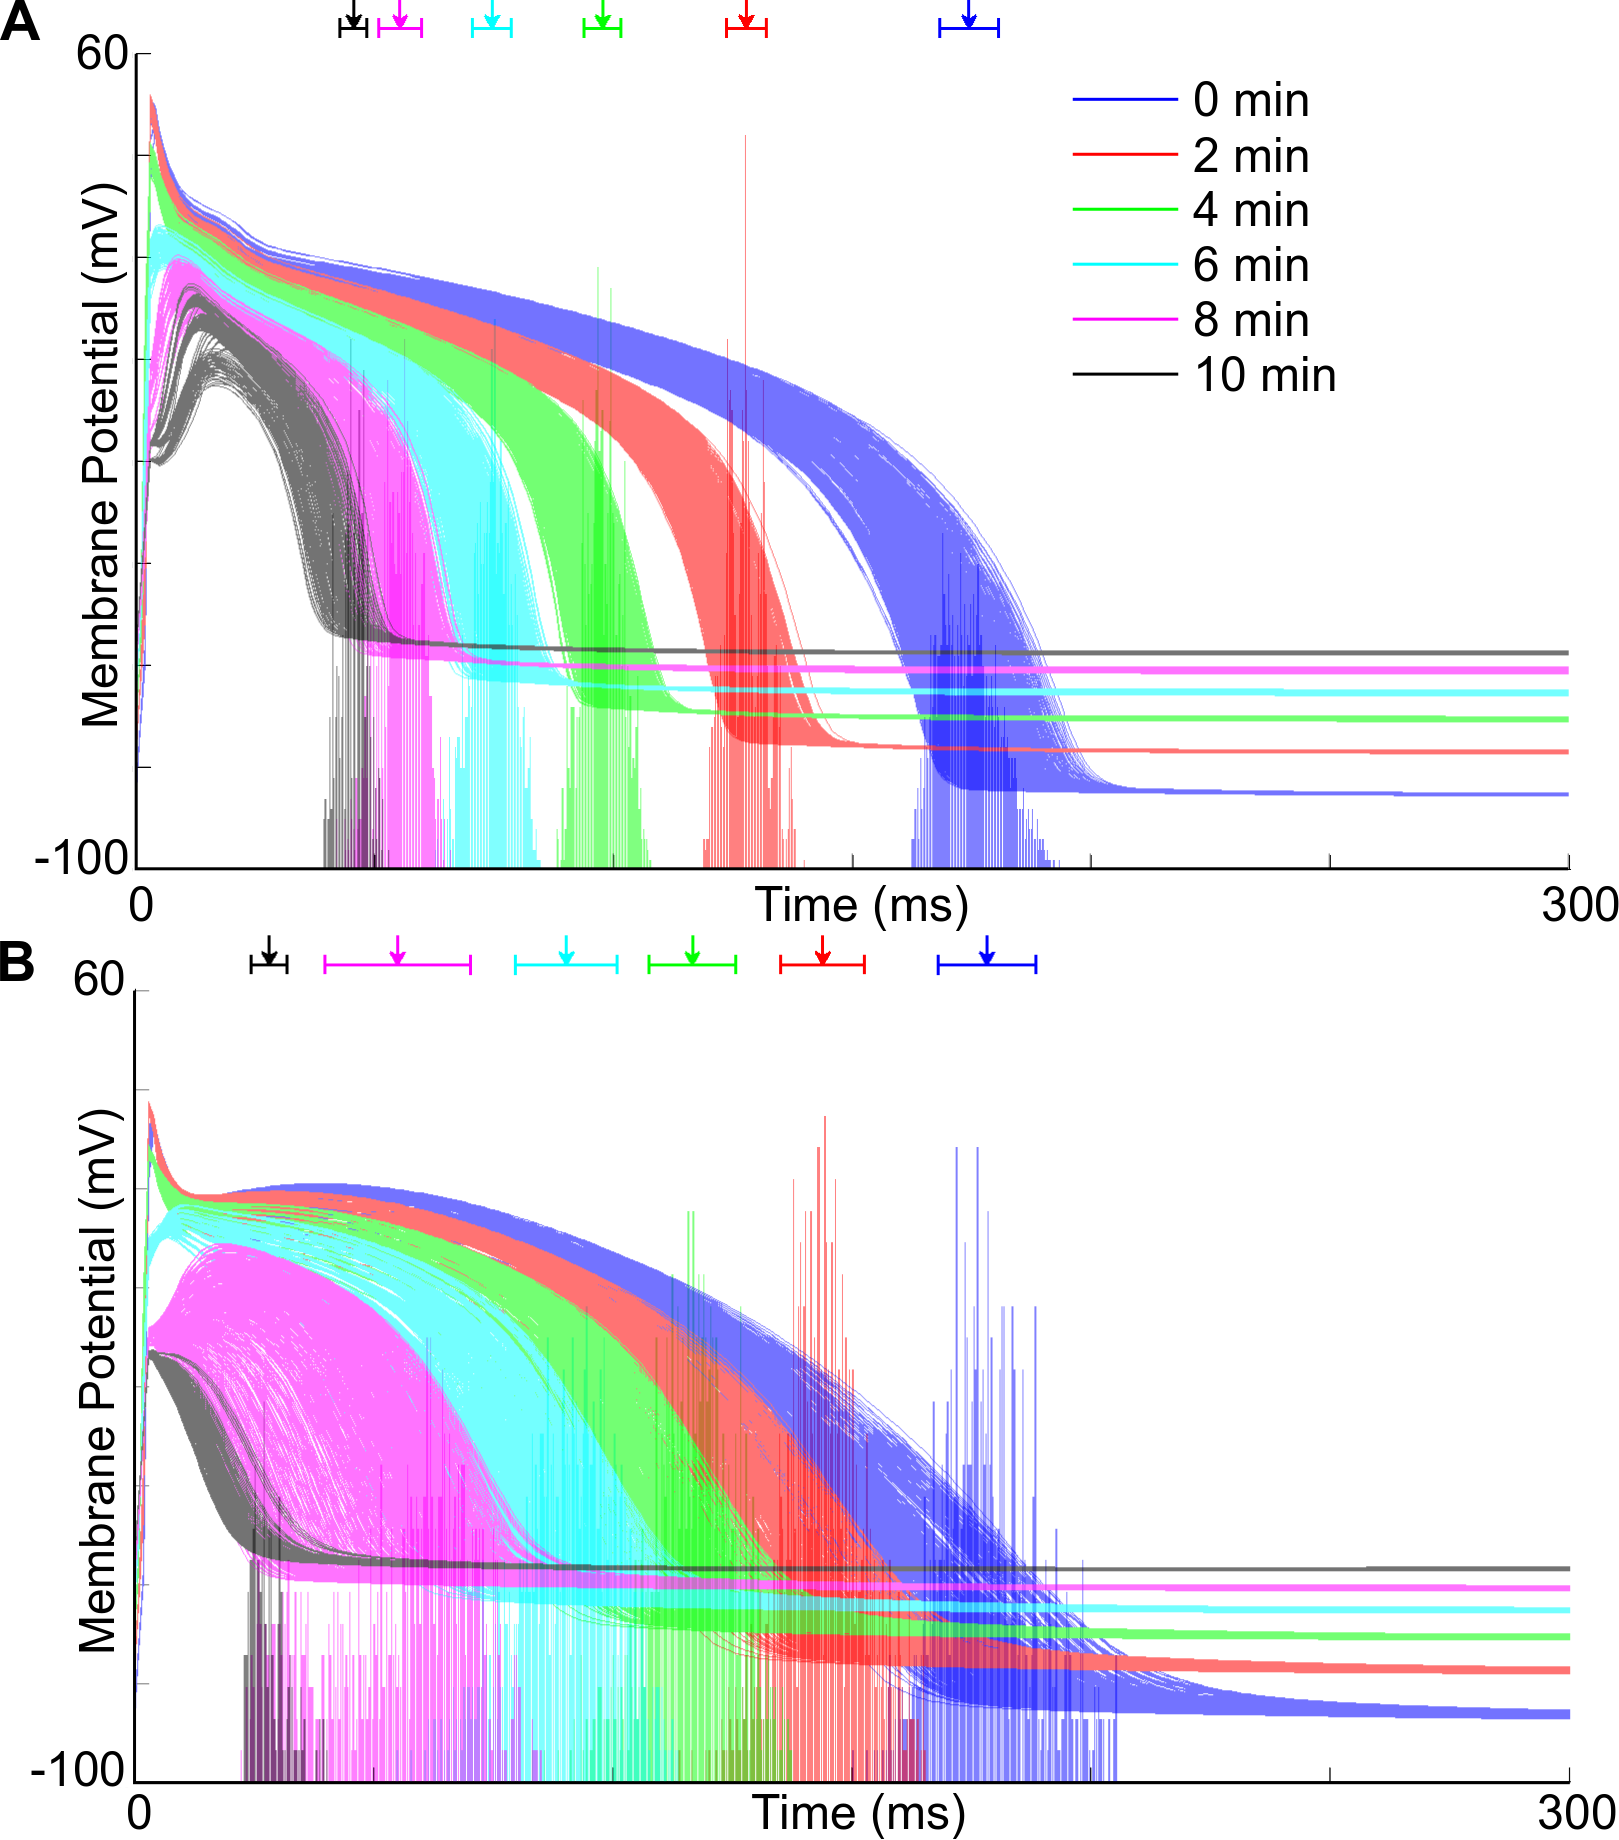
\includegraphics[width=0.8\textwidth]{isch-ap-apd90}
 \caption[Effect of different degrees of isch\ae{}mia on the Shannon and Mahajan model populations.]{Effect of different degrees of isch\ae{}mia on the Shannon (A) and Mahajan (B) model populations. The histograms respresent the APD\sub{90} values associated with the populations.}
 \label{fig:isch-ap-apd90}
\end{figure}

\subsection{APD\sub{90}}
\label{subsec:isch-apd90-response}
For both model populations, progression of isch\ae{}mia works to reduce populations variation in its early stages (until 4 min PO)---beyond this point, the response is population-dependent, as can be seen in Fig.~\ref{fig:isch-ap-apd90} and Table~\ref{table:isch-stats}.

% Data for [K+]o(isch) = 17 mM
% \begin{table}
%  \centering
%  \begin{tabular}{ccc|cccccc}
%   & & & \multicolumn{6}{c}{Time PO (min)} \\
%   & & & 0 & 2 & 4 & 6 & 8 & 10 \\
%   \hline
%   \hline
%   \multirow{9}{*}{Shannon} & \multirow{3}{*}{APD\sub{90}} & Mean & $174.1$ & $127.4$ & $97.4$ & $74.2$ & $55.0$ & $45.3$ \\
%   & & Std & $6.23$ & $4.17$ & $3.89$ & $4.14$ & $4.44$ & $2.82$ \\
%   & & Range & $30.9$ & $20.9$ & $19.7$ & $21.8$ & $23.5$ & $13.5$ \\
%   \cline{2-9}
%   & \multirow{3}{*}{ERP} & Mean & $175.9$ & $132.7$ & $107.5$ & $93.2$ & $94.8$ & $182.9$ \\
%   & & Std & $6.20$ & $4.21$ & $3.85$ & $3.77$ & $2.87$ & $31.47$ \\
%   & & Range & $30.7$ & $21.3$ & $19.5$ & $19.9$ & $15.5$ & $324.0$ \\
%   \cline{2-9}
%   & \multirow{3}{*}{PRR} & Mean & $1.8$ & $5.3$ & $10.1$ & $19.0$ & $39.8$ & $137.6$ \\
%   & & Std & $0.09$ & $0.19$ & $0.23$ & $0.49$ & $1.96$ & $31.94$ \\
%   & & Range & $0.4$ & $1.1$ & $1.1$ & $2.1$ & $8.2$ & $319.9$ \\
%   \hline
%   \multirow{9}{*}{Mahajan} & \multirow{3}{*}{APD\sub{90}} & Mean & $177.9$ & $143.6$ & $116.3$ & $90.0$ & $54.7$ & $27.8$ \\
%   & & Std & $10.20$ & $8.77$ & $9.04$ & $10.64$ & $15.25$ & $3.75$ \\
%   & & Range & $55.0$ & $51.4$ & $54.0$ & $58.4$ & $62.5$ & $17.4$ \\
%   \cline{2-9}
%   & \multirow{3}{*}{ERP} & Mean & $174.2$ & $148.7$ & $128.0$ & $112.0$ & $100.8$ & $600.0$ \\
%   & & Std & $9.32$ & $8.82$ & $9.43$ & $11.44$ & $18.31$ & $0.00$ \\
%   & & Range & $50.2$ & $51.4$ & $56.2$ & $63.3$ & $77.5$ & $0.0$ \\
%   \cline{2-9}
%   & \multirow{3}{*}{PRR} & Mean & $-3.7$ & $5.1$ & $11.7$ & $22.0$ & $46.1$ & $572.2$ \\
%   & & Std & $1.98$ & $0.32$ & $0.48$ & $0.91$ & $3.17$ & $3.75$ \\
%   & & Range & $7.9$ & $2.0$ & $2.3$ & $5.0$ & $15.5$ & $17.4$
%  \end{tabular}
%  \caption[Isch\ae{}mic Effect on Model Populations]{Effect of different degrees of isch\ae{}mic severity on the population level response for common biomarkers for the Mahajan and Shannon frameworks, according to mean, standard deviation (Std) and range.}
%  \label{table:isch-stats}
% \end{table}
% Mention importance of looking at overall population response, e.g. overall population spread via std or inspection of histograms. Massive increase in range many not be important...

\subsection{ERP and PRR}
\label{subsec:isch-erpprr-response}
% Limitations of ERP calculation for severe ischæmia (ERP > 600 ms)
% Very small variation in PRR => high correlation between APD90 and ERP, which declines with increasing ischæmic severity

\subsection{Other Biomarkers}
\label{subsec:isch-other-response}

\section{Effects within Isch\ae{}mic Parameter Space}
\label{sec:isch-space}
% Effect of I(K-ATP) on PRR (APD90 and ERP correlation)

\section{Model Failure During Isch\ae{}mia}
\label{sec:isch-modelFailure}

\biblio

\end{document}